\documentclass[conference]{IEEEtran}
\IEEEoverridecommandlockouts
% The preceding line is only needed to identify funding in the first footnote. If that is unneeded, please comment it out.
\usepackage{cite}
\usepackage{amsmath,amssymb,amsfonts}
\usepackage{algorithmic}
\usepackage{graphicx}
\usepackage{textcomp}
\usepackage{xcolor}
\usepackage[ngerman]{babel}
\usepackage[acronym]{glossaries}
\usepackage{url}
%\usepackage{setspace}
\makeglossaries
\newacronym{mri}{MRI}{Serious Games}


\def\BibTeX{{\rm B\kern-.05em{\sc i\kern-.025em b}\kern-.08em
    T\kern-.1667em\lower.7ex\hbox{E}\kern-.125emX}}
\begin{document}

\title{Implementation of an Open-Source modular mangetic field camera for usage in Low-Field MRI Systems}


\author{\IEEEauthorblockN{1\textsuperscript{st} Marcel Werner Heinrich Friedrich Ochsendorf}
\IEEEauthorblockA{\textit{Fachhochschule Aachen} \\
\textit{Electrical Engineering and Information Technology}\\
Aachen, Deutschland \\
marcelochsendorf@alumni.fh-aachen.de}
%\and
}

\maketitle

%-----------------------------------------------------------------------------------------------------------------------------------------------
% \gls{uscf}
\begin{abstract}

\end{abstract}

\begin{IEEEkeywords}
%Serious Gaming (\gls{sg}), \gls{vr}, Extended Reality (\gls{xr}), Computer Grafik (\gls{cg})
\end{IEEEkeywords}



% Introduction
%-----------------------------------------------------------------------------------------------------------------------------------------------
\section{Introduction}


\subsection{Use Cases}

% magnet measurements
% field visualisation
% static analysis
% CI based tests


% Hardware
%-----------------------------------------------------------------------------------------------------------------------------------------------


\section{Hardware}

% modular
% low cost
%easy to reproduce

\subsection{Sensor selection}
%tabelle möglicherdigitaler sensoren
% mixture of sensors
% tablee with ranges
% digital only at the moment
\subsection{Sensor slice}
% 
\begin{figure}[htbp]
\centerline{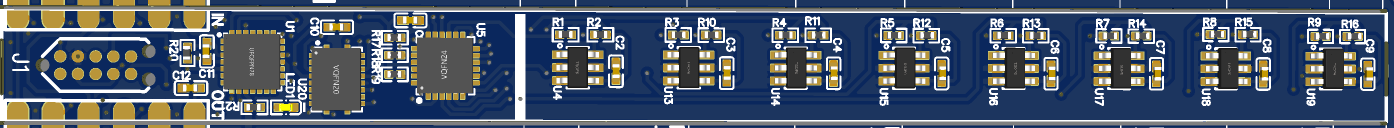
\includegraphics[width=8cm]{magcam_sensor_module.png}}
\caption{Sensor Slice with eight TLV493d sensors.\cite{magcam_sensor_module}}
\label{magcam_sensor_module_fig}
\end{figure}

\subsection{Communication bus}
To ensure modularity and easy expandability of the sensor system, it is necessary to be able to integrate several sensor slices into the system.
On the electrical level, a CAN bus was implemented to connect the individual microprocessors to which up to 16 magnetic field sensors can be digitally connected to an overall system.

In addition to the bus system, a supply voltage and a separate synchronisation signal are necessary to enable automatic recognition of connected sensors. This is connected in a daisy chain between the slices.
This enables the microcontroller of a sensor slice to recognise whether it is integrated into a network and to register itself via the system bus.



\subsection{Powermanagement}
sensor on off

\subsection{Sensor-Selection}
%tabelle möglicherdigitaler sensoren


\subsection{Mechanical integration}

% 3d printed cases for magnet holders
%
%-----------------------------------------------------------------------------------------------------------------------------------------------
% Embedded System Software
\section{Embedded System Software}

\subsection{Automatic Sub-Sensor Detection}



\subsection{Synchronisation}

In order to ensure synchronisation of all sensors in the array, in addition to the bus system used for data transmission, a clock line is shared between all sensors.
After performing the autonumbering procedure, the clock line, which was previously used as an autonumbering return channel, is reconfigured as a digital input.
This is done for all connected sensor modules except for the slices connected to the readout host system.
This module then specifies the read clock via this data line, which can be configured in the software.
All other sensors use this signal to trigger a readout interrupt.

This procedure also ensures that the rest of the system maintains a synchronised state even if sensor slices fail or are restarted.
Modules that fall into an out-of-sync status can thus be resynchronised directly after a synchronisation pulse.


%-----------------------------------------------------------------------------------------------------------------------------------------------
%Analysis Software Framework
\section{Analysis Software Framework}

The collection and subsequent processing of the data read from the sensor array is carried out on another computer system (host).
For this purpose, the Python framework is used, which was specially developed for the automated processing of magnetic field sensor data.
By adapting the sensor software on the basis of the documentation, a direct evaluation of the sensor is possible through the library.
Through the implemented auto-numbering routine and the feedback of this to the host software, each individual sensor is assigned to an individual measurement in the host software.

\subsection{Data analysis pipeline}





\subsection{Calibration Run}

cli einstellungen
+ ergebnis

\subsection{Measurement Run}





%-----------------------------------------------------------------------------------------------------------------------------------------------
%Evaluation

\section{Evaluation}

\subsection{Comparison}
% mit mechanischen aufbau
% durch feste positionen nur zurückrechenbar

%-----------------------------------------------------------------------------------------------------------------------------------------------
%Conclusion

\section{Conclusion}


%-----------------------------------------------------------------------------------------------------------------------------------------------
\begingroup
\begin{thebibliography}{00}
%\setstretch{1.05}
\bibitem{modhhsf} Marcel Ochsendorf: Development of a hardware and software framework for the automated characterization of permanent magnets for low-field MRI systems. Available: \url{https://www.researchgate.net/publication/374388764_Development_of_a_permanent_magnet_characterization_framework_for_use_in_low-field_MRI_systems}, 17.11.2021.

\vskip 0.05in
\bibitem{MagneticReadoutProcessingLib} Marcel Ochsendorf: MagneticReadoutProcessing-Framework. \url{https://github.com/LFB-MRI/MagneticReadoutProcessing}, 17.11.2021


\end{thebibliography}
\endgroup

\end{document}


